\documentclass[letterpaper,12pt]{article}
%\usepackage{fullpage}
\usepackage{geometry}
 \geometry{
 left=1in,right=1in,top=0.5in,bottom=0.5in
 }
\usepackage{tikz}
\tikzset{minimum size=0.8cm}
\usepackage{amsmath}
\usepackage{hyperref}
\usepackage{wrapfig}
\usepackage{mathtools}
\usepackage[group-minimum-digits={3}]{siunitx}
\pagenumbering{gobble}
\setcounter{MaxMatrixCols}{20}
\begin{document}

\begin{center} \textbf{Alex Ni, Math 2210 \\ Fall 2021 \\ Project 2 -- Studying Networks with Eigenvectors and Eigenvalules\\ }
\hrulefill
\end{center}


\subsubsection*{Introduction}
The project will consider the connectivity structure of the network of bus stops in the Ithaca TCAT system. We will see how the Fiedler Set of the network's Laplacian matrix splits the network in two between stops on Cornell University campus and the rest of Ithaca.

\subsubsection*{Network Description}
The network studied in this project is the network of buses that run throughout Ithaca. This bus system, part of Tompkins Consolidated Area Transit (TCAT), provides transportation to many residents in Ithaca and surrounding towns. I selected a subset of 12 bus stops that I believe Cornell students use most often during the academic year. Each node in the graph is a bus stop. There is an edge between two stops if they are directly adjacent stops for any of the bus routes (excluding other stops in between that I removed for simplification). The bus stops are, in order from 1-12, Shops at Ithaca Mall, RPCC, Helen Newman Rec Center, Risley Hall, Milstein Hall, Rockefeller Hall, Baker Flagpole, Uris Hall, Statler Hall, Anabel Taylor Hall, Collegetown, and Ithaca Commons. Their connections were taken from the up-to-date TCAT website.\footnote{\href{https://realtimetcatbus.availtec.com/InfoPoint/}{https://realtimetcatbus.availtec.com/InfoPoint/}}


\subsubsection*{Laplacian Matrix and Network Representation}
A Laplacian matrix of the network in question (on the right) is shown below. The $n$th diagonal entry represents the number of connections for the nth node. The $-1$s on the (i,j) and (j,i) entries represent a connection between nodes $i$ and $j$.


\begin{wrapfigure}[4]{r}[2pt]{-2cm} 
\centering
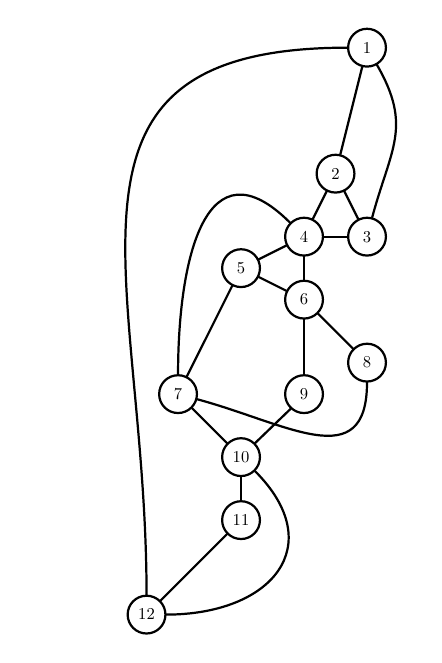
\begin{tikzpicture}[thick,scale=1, every node/.style={scale=0.6}]
    \node[shape=circle,draw=black] (A) at (2.8,7.2) {1};
    \node[shape=circle,draw=black] (B) at (2.4,5.6) {2};
    \node[shape=circle,draw=black] (C) at (2.8,4.8) {3};
    \node[shape=circle,draw=black] (D) at (2,4.8) {4};
    \node[shape=circle,draw=black] (E) at (1.2,4.4) {5};
    \node[shape=circle,draw=black] (F) at (2,4) {6} ;
    \node[shape=circle,draw=black] (G) at (0.4,2.8) {7};
    \node[shape=circle,draw=black] (H) at (2.8,3.2) {8};
    \node[shape=circle,draw=black] (I) at (2,2.8) {9};
    \node[shape=circle,draw=black] (J) at (1.2,2) {10};
    \node[shape=circle,draw=black] (K) at (1.2,1.2) {11};
    \node[shape=circle,draw=black] (L) at (0,0) {12};

    \draw (A) -- (B);
    \draw (A) edge[out=300,in=75,looseness=1.2] (C);
    \draw (A) edge[out=180,in=90,looseness=1.4] (L);
    \draw (B) -- (C);
    \draw (B) -- (D);
    \draw (C) -- (D);
    \draw (D) -- (E);
    \draw (D) -- (F);
    \draw (D) edge[out=135,in=90,looseness=1.6] (G);
    \draw (E) -- (F);
    \draw (E) -- (G);
    \draw (F) -- (H);
    \draw (F) -- (I);
    \draw (G) edge[out=345,in=270,looseness=1.4] (H);
    \draw (G) -- (J);
    \draw (I) -- (J);
    \draw (J) -- (K);
    \draw (J) edge[out=315,in=0,looseness=1.6] (L);
    \draw (K) -- (L);
\end{tikzpicture}
\caption{TCAT Network at Cornell}
\end{wrapfigure}

\begin{align*}
\begin{bmatrix}
3 & -1 & -1 & 0 & 0 & 0 & 0 & 0 & 0 & 0 & 0 & -1\\
-1 & 3 & -1 & -1 & 0 & 0 & 0 & 0 & 0 & 0 & 0 & 0\\
-1 & -1 & 3 & -1 & 0 & 0 & 0 & 0 & 0 & 0 & 0 & 0\\
0 & -1 & -1 & 5 & -1 & -1 & -1 & 0 & 0 & 0 & 0 & 0\\
0 & 0 & 0 & -1 & 3 & -1 & -1 & 0 & 0 & 0 & 0 & 0\\
0 & 0 & 0 & -1 & -1 & 4 & 0 & -1 & -1 & 0 & 0 & 0\\
0 & 0 & 0 & -1 & -1 & 0 & 4 & -1 & 0 & -1 & 0 & 0\\
0 & 0 & 0 & 0 & 0 & -1 & -1 & 2 & 0 & 0 & 0 & 0\\
0 & 0 & 0 & 0 & 0 & -1 & 0 & 0 & 2 & -1 & 0 & 0\\
0 & 0 & 0 & 0 & 0 & 0 & -1 & 0 & -1 & 4 & -1 & -1\\
0 & 0 & 0 & 0 & 0 & 0 & 0 & 0 & 0 & -1 & 2 & -1\\
-1 & 0 & 0 & 0 & 0 & 0 & 0 & 0 & 0 & -1 & -1 & 3
\end{bmatrix}
\end{align*}
\begin{center} Laplacian Matrix for Fig. 1
\end{center}

\clearpage

\begin{center} \underline{    Alex Ni, Project 2 - Studying Networks with Eigenvectors and Eigenvalules - Page 2 of 2    }

\end{center}

\subsubsection*{Fiedler Eigenvector, Eigenvalue, and Fiedler Set}
We can see visually from the network that it is connected, meaning that the Fiedler value $\lambda_{2}$ is greater than zero, so the multiplicity of the eigenvalue 0 is just one. We therefore do not need to add any more edges to the network to make it connected.

\noindent Using an online Julia calculator\footnote{\href{https://www.tutorialspoint.com/execute\_julia\_online.php}{https://www.tutorialspoint.com/execute\_julia\_online.php}}, we compute that $\lambda_{2} = 0.76905 > 0$ and find that the Fiedler vector is (split into two rows for fit):

\begin{align*}
\begin{bmatrix} -0.283388 & -0.109245 & -0.109245 & 0.148913 & 0.308716 & 0.314283 \end{bmatrix} \\
\begin{bmatrix} 0.225535 & 0.438537 & 0.119265 & -0.167473 & -0.472163 & -0.413736 \end{bmatrix}.
\end{align*}

\noindent Taking all the positive values, we see that the Fiedler set is:

$$F = \{4, 5, 6, 7, 8, 9\}$$


\subsubsection*{Analysis and Discussion}

\noindent Looking only the graph, observe that there are only 4 edges between the Fiedler set and the rest of the graph. Since the Fiedler set has 6 nodes and the entire network has 12, this splits the network into two groups of the same size. The low number of edges crossing the Fiedler set to the rest of the graph shows that there is a clear separation between the set and the rest of the graph. Through observation, we see that the Fieder set corresponds to the bus stops on central campus, while the rest of the graph includes north campus and other regularly visited parts of Ithaca. This makes sense, as there are two main bridges that cross from central to south campus, and central to north campus. Thus, buses would only be able to take a select few routes to enter and exit central campus. \\

\noindent Of the vectors in the Fiedler set, we see that nodes 4 and 9 are closest to zero, which means they could be on either side of the split. These correspond to the stops close to the north bridge and south bridge of central campus, respectively. For further investigation, the other bus stops could be considered, though this would lead to a much more loosely connected graph (many two connections).
\end{document}
















